\documentclass[tikz, border=5mm]{standalone}
\usepackage{textcomp}
\usetikzlibrary{arrows.meta,decorations.markings,fit,calc, positioning}

\definecolor{componentColor}{RGB}{210,210,210}
\definecolor{systemColor}{RGB}{230,230,230}

\tikzset{component/.append style={fill=componentColor, align=center, draw, minimum width=2cm, minimum height=1.5cm, rounded corners=.3cm}}
\tikzset{system/.style={component, fill=systemColor, rounded corners=0cm}}


\begin{document}

	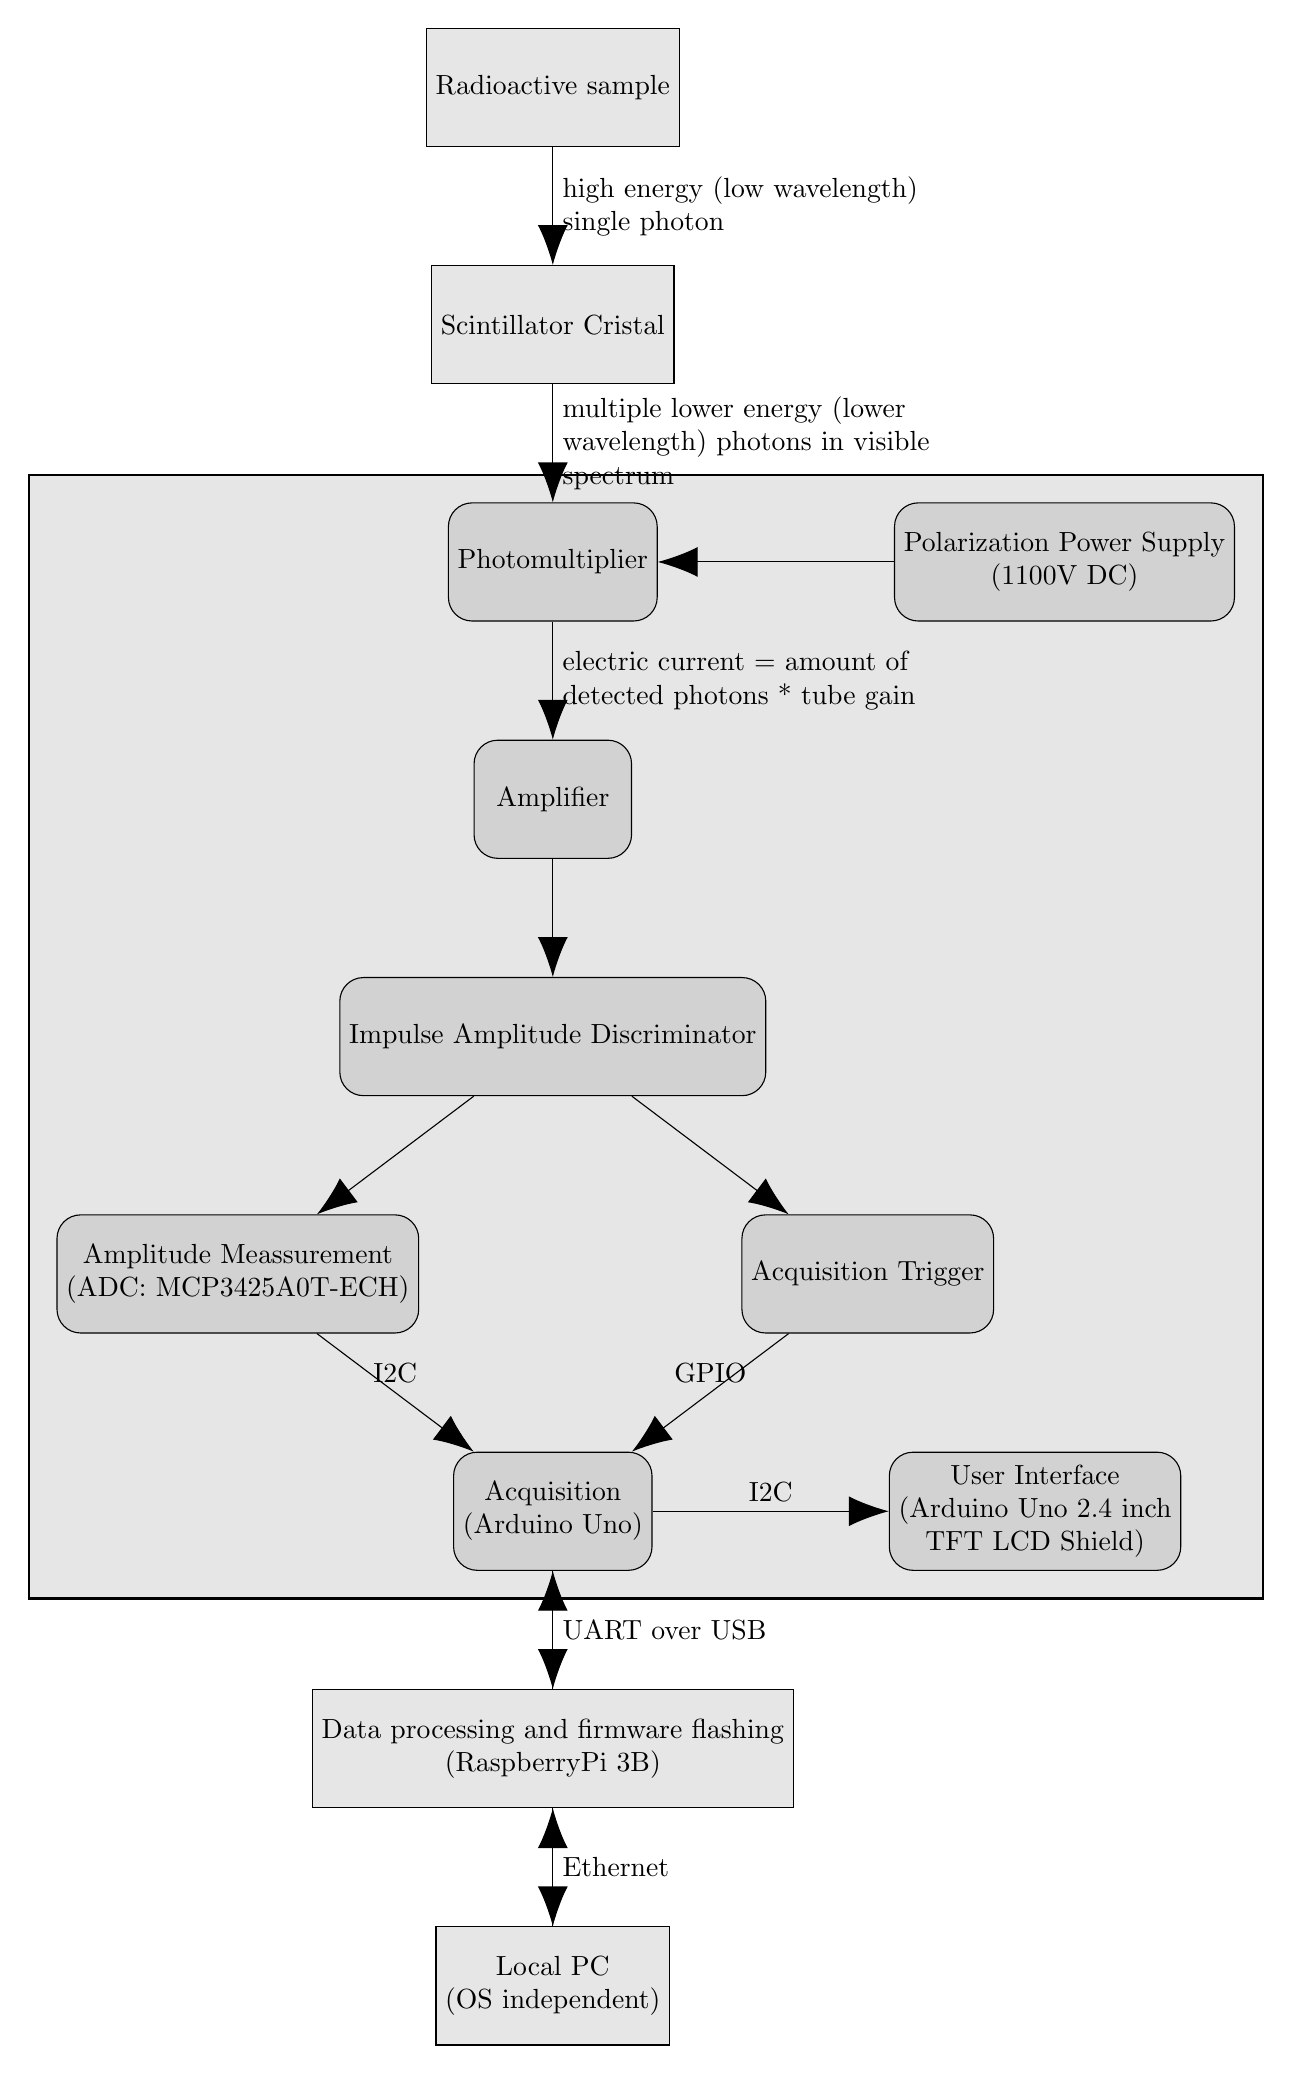
\begin{tikzpicture}[node distance=1.5cm and 3cm]
	% Nodes
	\pgfdeclarelayer{background}
	\pgfsetlayers{background,main}
	
		\node (sample) [system] {Radioactive sample};
		\node (scintillatorcristal) [system, below=of sample] {Scintillator Cristal};
		\node (photomultiplier) [component, below=of scintillatorcristal] {Photomultiplier};
		
		
		\node (hwpower) [component, right=of photomultiplier] {Polarization Power Supply\\ (1100V DC)};
		\node (amplifier) [component, below=of photomultiplier] {Amplifier};

		\node (discriminator) [component, below=of amplifier] {Impulse Amplitude Discriminator};

		\node (peakssurement) [component, below=of discriminator, xshift=-4cm] {Amplitude Meassurement\\  (ADC: MCP3425A0T-ECH)};
		\node (trigger) [component, below=of discriminator, xshift=4cm] {Acquisition Trigger};

		\node (cpu) [component, below=of peakssurement, xshift=4cm] {Acquisition\\ (Arduino Uno)};
		\node (gui) [component, right=of cpu] {User Interface\\ (Arduino Uno 2.4 inch \\ TFT LCD Shield)};
			
		\node (pi) [system, below=of cpu] {Data processing and firmware flashing\\ (RaspberryPi 3B)};
		\node (pc) [system, below=of pi] {Local PC\\ (OS independent)};
		
		\begin{pgfonlayer}{background}
		\node[system, draw, thick, inner xsep=1em, inner ysep=1em, fit= (photomultiplier) (hwpower) (amplifier) (discriminator) (peakssurement) (trigger) (cpu)] {};
		\end{pgfonlayer}
		
		% Connectors
		\begin{scope}[->]
		
		\draw [-{Latex[scale=3.0]}] (sample) -- node[anchor=west, minimum width=.25cm, draw=none, text width=5.0cm] 
			{high energy (low wavelength) single photon} (scintillatorcristal);

		\draw [-{Latex[scale=3.0]}] (scintillatorcristal) -- node[anchor=west, minimum width=.25cm, draw=none, text width=5.0cm] 
			{multiple lower energy (lower wavelength) photons in visible spectrum} (photomultiplier);

		\draw [-{Latex[scale=3.0]}] (hwpower) -- node[anchor=south, minimum width=.25cm, draw=none] {} (photomultiplier);

		\draw [-{Latex[scale=3.0]}] (photomultiplier) -- node[anchor=west, minimum height=.25cm, draw=none, text width=5.0cm, minimum height=2cm, ] 
			{electric current = amount of detected photons * tube gain} (amplifier);

		\draw [-{Latex[scale=3.0]}] (amplifier) -- node[anchor=west, minimum height=.25cm, draw=none] {} (discriminator);

		\draw [-{Latex[scale=3.0]}] (discriminator) -- node[anchor=south, minimum height=.25cm, draw=none] {} (trigger);
        \draw [-{Latex[scale=3.0]}] (discriminator) -- node[anchor=south, minimum height=.25cm, draw=none] {} (peakssurement);

		\draw [-{Latex[scale=3.0]}] (peakssurement) -- node[anchor=south, minimum height=.25cm, draw=none] {I2C} (cpu);
		\draw [-{Latex[scale=3.0]}] (trigger) -- node[anchor=south, minimum height=.25cm, draw=none] {GPIO} (cpu);

		\draw [-{Latex[scale=3.0]}] (cpu) -- node[anchor=south, minimum height=.25cm, draw=none] {I2C} (gui);

		\draw [-{Latex[scale=3.0]}] (cpu) -- node[anchor=west, minimum height=.25cm, draw=none] {UART over USB} (pi);
		\draw [-{Latex[scale=3.0]}] (pi) -- node[anchor=south, minimum height=.25cm, draw=none] {} (cpu);

		\draw [-{Latex[scale=3.0]}] (pi) -- node[anchor=west, minimum height=.25cm, draw=none] {Ethernet} (pc);
		\draw [-{Latex[scale=3.0]}] (pc) -- node[anchor=west, minimum height=.25cm, draw=none] {} (pi);
	
	\end{scope}

\end{tikzpicture}
\end{document}
